\documentclass{newsletter_2025}

\usepackage{multirow}
\usepackage{tabularx}

\graphicspath{ {./obrazky/} }

\kdrtitle{Leden 2025}
\kdrsubtitle{Newsletter komise rozhodčích a delegátů}
\kdrbackground{listopad-2024-background.jpg}

\begin{document}

\kdrtoc
\pagebreak
\clanek{Vážení rozhodčí a delegáti}
Dovolte mi vás přivítat u lednového newsletteru od KRD USaLB. Omlouváme se za delší prodlevu od předchozího vydání, ale  věříme, že nyní již pojedeme opět pravidělně. Připravili jsme si pro vás pestrou škálu témat, která se týkají pravidel a prací se elektronickým zápisem o utkání (EZOU), ve které došlo nedávno ke změnám. Věříme, že vás jednotlivá témata zaujmou a pomohou Vám lépe zvládat specifické situace na hřišti i mimo něj.

KRD bude opět ráda za jakoukoliv zpětnou vazbu, která nám pomůže vylepšit newslettery do budoucna tak, aby Vám co nejlépe pomáhali při činnosti rozhodčích a delegátů.

S přátelským pozdravem,

\begin{flushleft}
	\vspace{3\baselineskip}
	
\includegraphics[width=3.5cm, keepaspectratio]{tadeas_sidenberg_podpis}\\
	\textbf{Tadeáš Sidenberg}\\
	předseda KRD USaLB
\end{flushleft}

\pagebreak
\rubrika{cfred}{Aplikace pravidel}

\clanek{Bránění při výhozu}
KDR chce tímto připomenou dřívější výklad pravidla 507/10 a 605/11, která se týkají bránění brankáři ve výhozu. Za přestupek je považováno, pokud je hráč ve velkém brankovišti nebo blíže než 3 metry od brankáře, měřeno od místa, kde brankář získá kontrolu nad míčkem.

\begin{itemize}
	\item \textbf{Pasivní bránění} znamená neúmyslné, nebo pokud opomene uhnout. V takovém případě je podle pravidla 507/10 nařízen volný úder.
	\item \textbf{Aktivní bránění} znamená sledování pohybu brankáře nebo snahu získat míč florbalkou. V tomto případě je podle pravidla 605/11 udělen menší trest.
\end{itemize}

\clanek{Neopatrná a bezohledná hra florbalkou}
KRD vám tímto upřesňuje aplikace pravidel při hře florbalkou. Jedná se především o situace, které jsou považovány za neopatrné a které za bezohledné.

\begin{itemize}
	\item \textbf{Neopatrná hra florbalkou} vzniká v přirozených herních situacích, kdy je florbalka použita správným způsobem, ale dojde k přestupku. Jedná se tak například o nekontrolovaný nápřah nebo došvih.
	\item \textbf{Bezohledná hra florbalkou} vzniká v méně přirozených herních situacích, kdy florbalka není použita správným způsobem ke hře.
\end{itemize}

KRD připomíná, že při posuzování přestupků florbalkou i tělem by rozhodčí měl zvažovat několik faktorů, které do zákroků vstupují. Jejich správné hledání a posuzování je součástí vzdělávacích seminářů rozhodčích, ovšem jedná se zejména o \textbf{rychlost}, \textbf{sílu}, \textbf{kontakt}, \textbf{směr}, \textbf{úmysl} a \textbf{výsledek}.

\clearpage
\clanek{Potyčky hráčů a zapojení střídačky}
KDR vám tímto připomíná pravidlo 614/10, podle kterého je zapojení kohokoliv ze střídačky nebo trestné lavice do potyčky přestupkem, který je trestán udělením červené karty (TDKU).

\begin{admonition-quote}{614 Přestupky vedoucí k trestu do konce utkání}
	\begin{enumerate}\addtocounter{enumi}{9}
		\item \textbf{Opustí-li hráč nebo člen realizačního týmu prostor pro střídání nebo trestnou lavici, aby se zapojil do potyčky.}
		
		\begin{flushleft}
			Zapojením se rozumí situace, kdy se hráč nebo člen realizačního týmu fyzicky nebo slovně zapojí do potyčky se
			soupeřem nebo během potyčky přistoupí k rozhodčím.
		\end{flushleft}
	\end{enumerate}
\end{admonition-quote}

\textbf{Pokud můžete do daného konfliktu zasáhnout a ukončit jej, udělejte tak!} Jeden rozhodčí by měl aktivně pracovat na ukončení konfliktu, zatímco druhý zajišťuje, aby do situace nevstupovali další hráči, a zároveň sleduje, kdo a za co bude potrestán. V případě rozsáhlejšího konfliktu oba rozhodčí zůstávají v bezpečné vzdálenosti a věnují se pozorování situace, aby mohli rozhodnout o trestech. 

Příklad takové situace je ve \href{https://www.ceskyflorbal.cz/data/document/20240902/171344_86ae_Slozka-rozhodciho.pdf}{Složce rozhodčího}. Obrázek níže ilustruje situaci, kdy R2 zasahuje u ohniska konfliktu a odděluje hráče, zatímco R1 pozorně sleduje, kdo bude za co potrestán.

\begin{figure}[h]
	\centering
	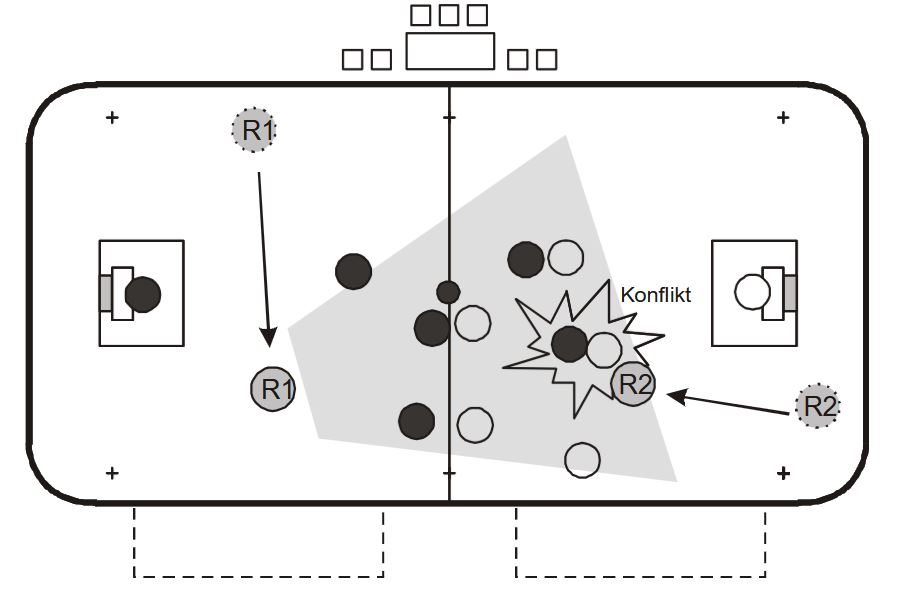
\includegraphics[width=0.85\textwidth, keepaspectratio]{konflikt}
\end{figure}

\clearpage
KRD doporučuje rozhodčím mít nastudovaný postup pro zapisování osobních trestů (OS), trestů do konce utkání (TDKU) a technického trestu (TT). Může se Vám totiž snadno stát, že zapisovatel si nebude vědět rady. Postup pro práci se ZOU najdete opět ve \href{https://www.ceskyflorbal.cz/data/document/20240902/171344_86ae_Slozka-rozhodciho.pdf}{Složce rozhodčího}, ovšem ve zkratce je potřeba trest rozepsat do dvou řádků:
\begin{itemize}
	\item Na prvním řádku je zapsáno vyloučení na trestnou lavici
	\item Na druhém řádku je zapsán dodatečný trest (osobní / technický / do konce utkání) 
\end{itemize}
KRD připomíná, že v aktuální verzi FISu nejde členovi realizačního týmu zapsat vyloučení na trestnou lavici. V případě udělení OS, TDKU nebo TT členovi realizačního týmu vždy vyloučení na trestnou lavici připisujte hráči, který ho na trestné lavici odslouží.

\begin{figure}[h]
	\centering
	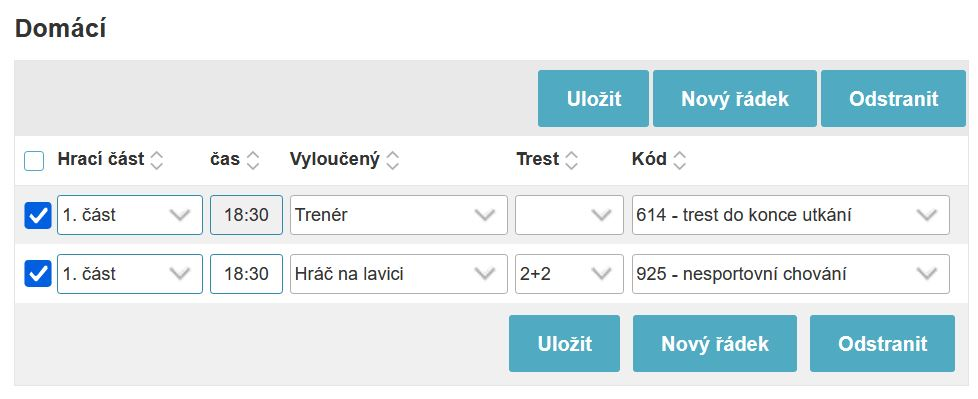
\includegraphics[width=0.85\textwidth, keepaspectratio]{zapsani_tdku_trener}
\end{figure}


\clearpage
\rubrika{cfblue}{Zápis o utkání}
\clanek{Novinky a změny v elektronickém zápise}

KRD si tímto dovoluje připomenout změny a novinky v systému elektronických zápisů o utkání, o kterých vám přišel e-mail od koordinátora regionu. Velkých změn dostála kolonka rozhodčích a hlavička zápisu, proto KRD doporučuje se rozhodčím s těmito změnami obeznámit, aby nedocházelo k problémům se zápisy.

Nejvýznamnější změny dostála záložka \textbf{Rozhodčí}, kde se dvoustavové zaškrtávací pole nahradilo třístavovým výběrem. Při vytvoření zápisu jsou tato pole prázdná, a je na vás jakožto rozhodčích ručně jít a vybrat, zda-li má být hodnota \textit{ano} či \textit{ne}. Pokud nějaké pole nezaškrtnete, budete na to upozorněni při ukončování zápisu. Změny dostálo i pole \textit{Rozměry hřiště}, kdy do polí lze nyní vepisovat desetinná čísla.

\begin{figure}[h]
	\centering
	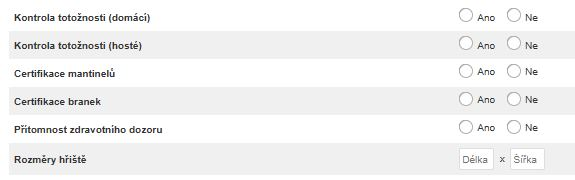
\includegraphics[width=0.85\textwidth, keepaspectratio]{nevyplneny_rozhodci}
\end{figure}

Se změnami polí přibyly i nové chyby, na které vás při ukončení utkání FIS upozorní. Jedná se zejména o nevyplněné kolonky v záložce rozhodčí (rozměr hřiště, certifikace mantinelů, branek a přítomnost zdravotního dozoru), nevyplněný čas konce utkání, jméno časoměřiče a hlavního pořadatele a počet přesilovek.

\begin{figure}[h]
	\centering
	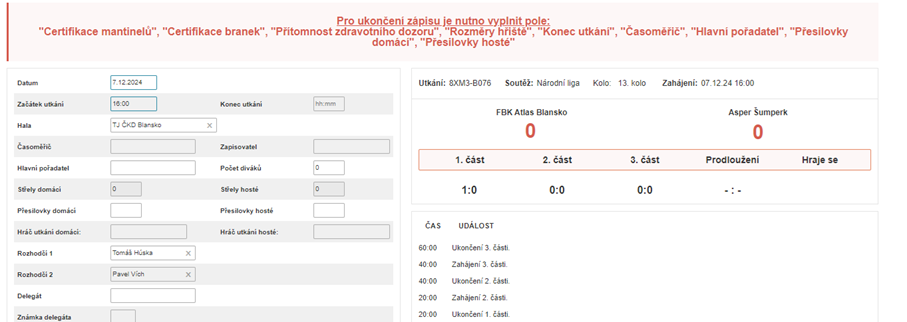
\includegraphics[width=0.85\textwidth, keepaspectratio]{nove_kontroly}
\end{figure}

\clearpage
\clanek{Doplnění hráče do EZOU}{}
KRD reaguje na dotazy ze strany rozhodčích nováčků a přináší vám návod, jak připsat hráče do zápisu o utkání. Hráče do zápisu o utkání můžeme doplnit pouze v případě, že utkání ještě nebylo zahájeno nebo je hráč doplněn za účelem udělení technického trestu (neuvedení v sestatě).

Postup pro doplnění hráče do soupisky je následující:
\begin{enumerate}
	\item Zjistěte jméno, příjmení, číslo dresu a datum narození hráče.
	\item Ujistěte se, že v hlavičce zápisu je odškrtlé zaškrtávací políčko \textbf{Zkontrolovat zápis}.\textit{ Pokud není, odškrtněte ho a klikněte \textbf{Uložit}}.
	\begin{figure}[h]
		\centering
		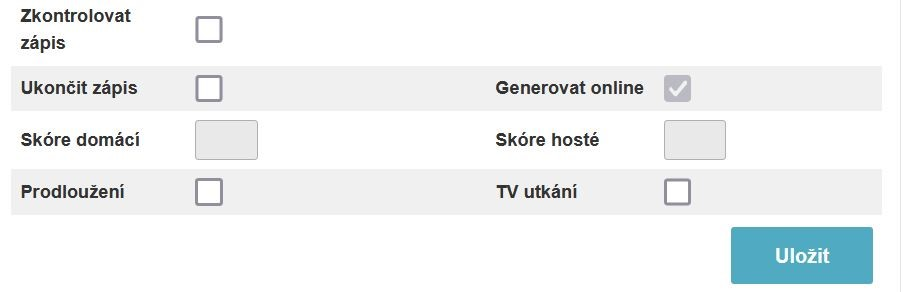
\includegraphics[width=0.85\textwidth, keepaspectratio]{zkontrolovat_zapis}
	\end{figure}
	\item Překlikněte se do záložky \textbf{Sestavy týmů}
	\item Pro přidání hráče máte tři možnosti. Rozdíl mezi polem \textbf{Vyberte hráče} a tlačítky \textbf{Hráči z oddílu} a \textbf{Všichni hráči z FISu} je pouze v zužení výsledků vyhledávání. Pokud si nejste jisti, používejte tlačítko \textbf{Všichni hráči z FISu}.
	\begin{figure}[h]
		\centering
		
\includegraphics[width=0.85\textwidth, keepaspectratio]{vyber_hrace_soupiska}
	\end{figure}
	\clearpage
	\item Vyhledejte hráče podle jeho jména a data narození. Pokud je hráčovo jméno ve vyhledávání
	\begin{itemize}
		\item zbarvené \textbf{černě}, klikněte na jeho jméno a přidejte ho do sestavy.
		\item zbarvené \textcolor{cfred}{\textbf{červeně}}, nemá uhrazený členský poplatek a nemůžete ho tak přidat do sestavy.
	\end{itemize}
	\begin{figure}[h]
		\centering
		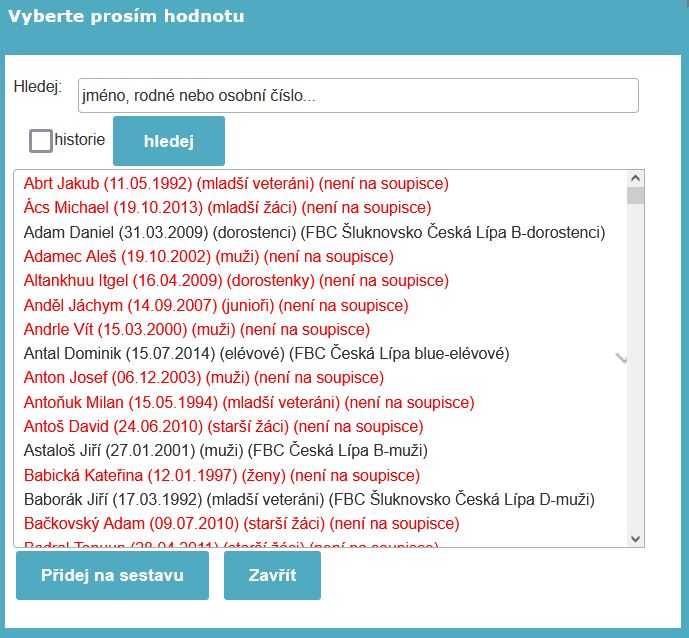
\includegraphics[width=0.6\textwidth, keepaspectratio]{vyber_hrace_z_fisu}
	\end{figure}
	\item Po kliknutí se hráč přidá do sestavy bez čísla. Doplňte číslo dresu tak, aby odpovídalo skutečnosti.
	\item Zkontrolujte záložku \textbf{Kontrola zápisu}, zda-li nevznikl koflikt s legislativními předpisy (např. porušení pravidla 2+1 či hraní za dvě družstva stejné soutěže v tentýž den).
\end{enumerate}

KRD dále upozorňuje, že pokud hráč, který není uveden v zápise o utkání, vstřelí branku, je tato branka podle pravidla 702/3 považována za správně vstřelenou. Je tedy nutné hráče podle výše uvedeného postupu přidat do zápisu o utkání, připsat mu vstřelenou branku a ve stejném čase udělit technický trest.

\begin{admonition-quote}{702 Správně vstřelené branky}
	\begin{enumerate}\addtocounter{enumi}{2}
		\item \textbf{Když se hráč, který není uveden v zápise o utkání, podílí na vstřelení branky}
		
		\begin{flushleft}
			Podílením se myslí vstřelení branky nebo asistence.
		\end{flushleft}
	\end{enumerate}
\end{admonition-quote}

\clearpage
\clanek{Pravidlo 2+1}{Výklad pravidla o startu hráčů}
KRD chce tímto způsobem rozhodčím a delegátům přiblížit pravidlo o startu hráčů za různá družstva svého oddílu, které je lidově známo jako pravidlo 2+1. Toto pravidlo říká, že pokud má oddíl v jedné věkové kategorii více týmů, může do sestavy za jeden tým zapsat nejvýše dva hráče v poli a jednoho brankáře z ostatních týmů v této kategorii. Smyslem tohoto pravidla je předejít situacím, kdy hráči z vyšších soutěží nastupují v těch nižších a vytváří tak neférové podmínky pro ostatní družstva v nižší soutěži.

\begin{admonition-quote}{5.3 Start hráčů za různá družstva svého oddílu}
	\begingroup
	\renewcommand{\theenumi}{\alph{enumi}}
	\begin{enumerate}\addtocounter{enumi}{2}
		\item Za družstvo mohou nastoupit v jednom soutěžním utkání vždy dva hráči dané věkové
		kategorie z každé jiné soupisky jiných družstev téhož oddílu startujících ve stejné
		věkové kategorii. Za družstvo může nastoupit i třetí hráč dané věkové kategorie ze
		soupisek jiných družstev téhož oddílu startujících ve stejné věkové kategorii v případě,
		že tento hráč startuje jako brankář.
	\end{enumerate}
	\endgroup
\end{admonition-quote}

FIS v aktuální verzi kontroluje pouze počet hráčů z jiných soupisek, ale nezjišťuje, zda tyto soupisky patří do stejné věkové kategorie. Pokud FIS najde více hráčů z jiných soupisek, upozorní na tuto chybu při kontrole zápisu.

\begin{figure}[h]
	\centering
	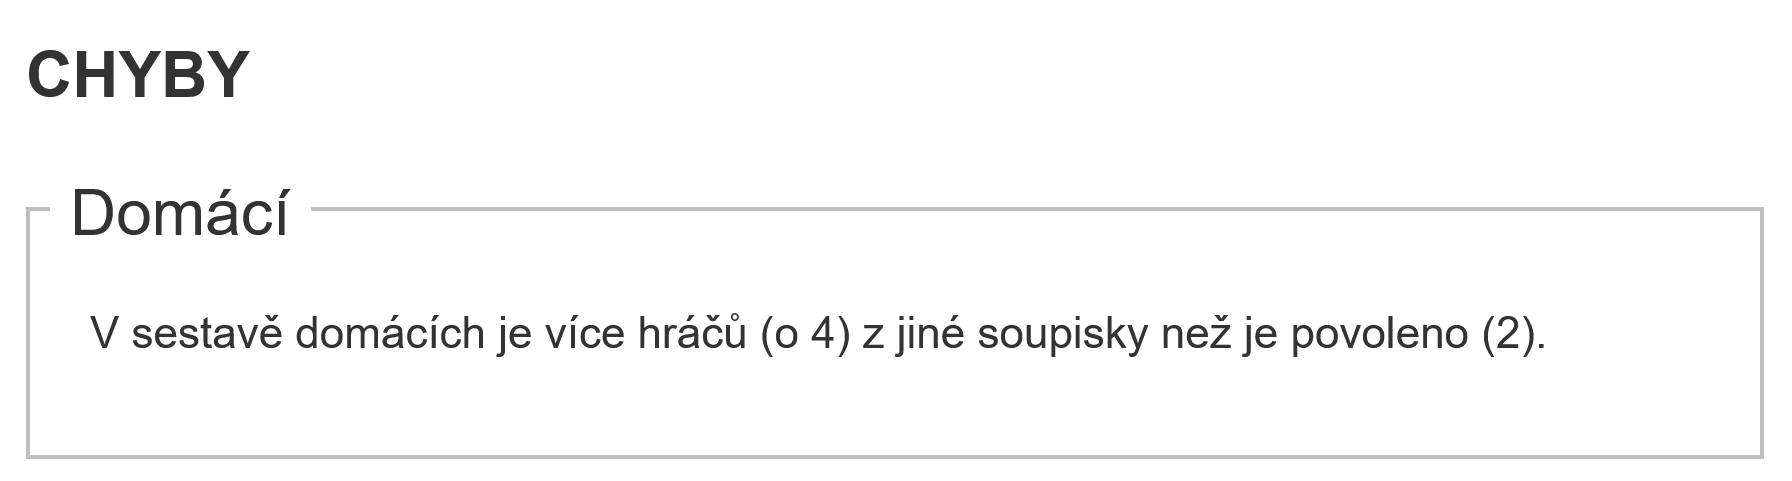
\includegraphics[width=0.8\textwidth]{chyba_pravidlo_2_1}\linebreak
	{\small\centering{Chyba v kontrole zápisu upozorňující na možné porušení pravidla 2+1}}
\end{figure}

\textbf{Jak postupovat při této chybě?}
\begin{itemize}
	\item Nalezněte hráče v sestavě, kteří toto pravidlo porušují
	\item Zkontrolujte, z jakých soupisek daní hráči pocházejí
	\item Pokud pochází ze soupisky ve stejné věkové kategorii, řešte tento problém s vedoucím družstva.
	\item Pokud pochází z jiných soupisek, a věkovou kategorii splňují, nemusíte tento problém řešit.
\end{itemize}

\begin{admonition-info}{Ilustrativní Příklad}
	\textbf{V kategorii dorostenek hraje domácí oddíl D proti hostujícímu oddílu H. Oba oddíly mají v kategorii dorostenek přihlášené jedno družstvo. Při kontrole zápisu rozhodčí zjistí, že vznikla chyba "V sestavě domácích je více hráčů (o 4) z jiné soupisky než je povoleno (2)". Jak rozhodčí situaci vyřeší?}
	
	\vspace{\baselineskip}
	Prvním krokem je zkontrolovat sestavu družstva v záložce \textbf{Sestavy týmů}. Rozhodčí musí identifikovat, které hráčky dané pravidlo porušují.
	
	\begingroup{\centering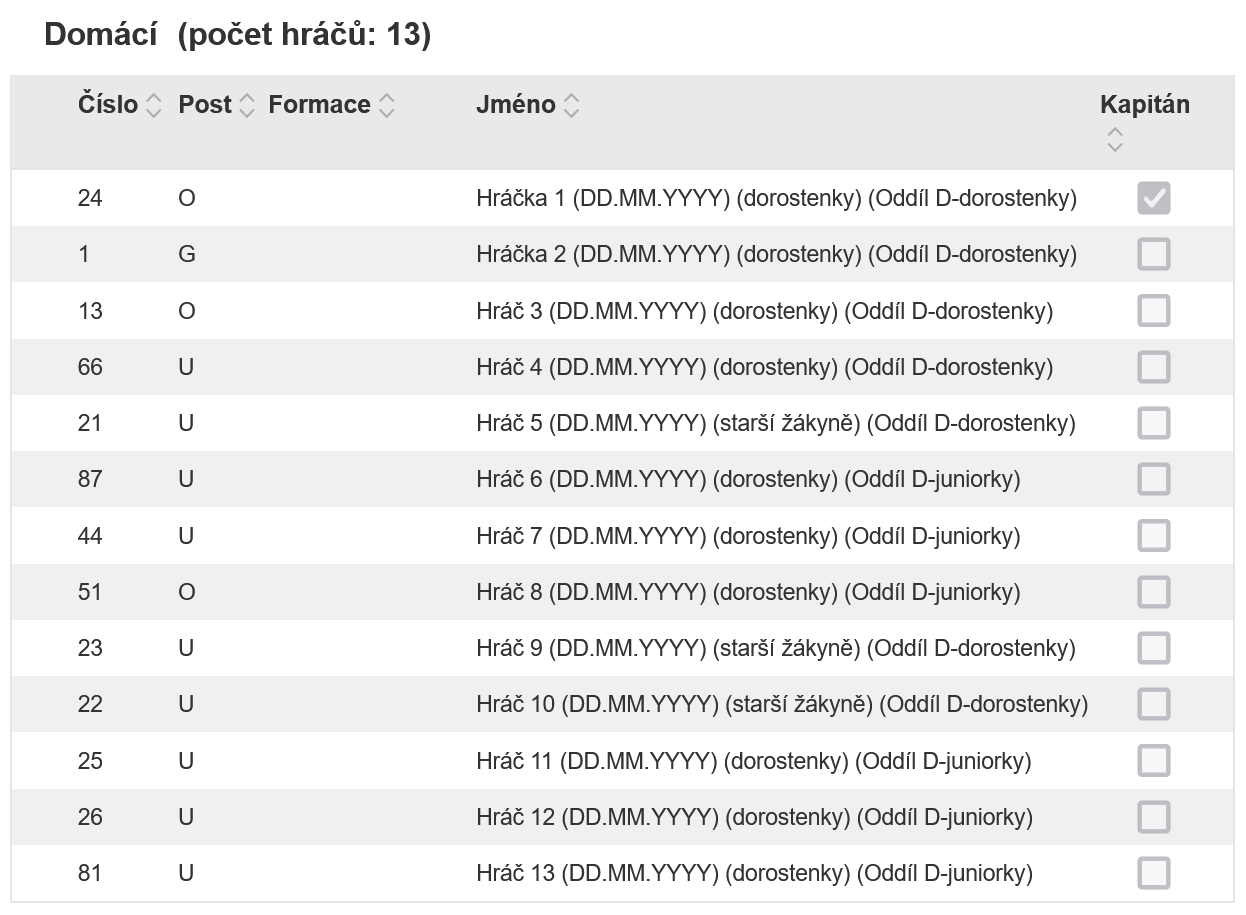
\includegraphics[width=0.65\textwidth]{soupiska_priklad}}\endgroup
	
	V tomto případě se jedná o hráčky ze soupisky juniorek. Těchto hráček je v sestavě domácího oddílu 6 a FIS kontroluje počet hráčů z jiných soupisek. Hráčky jsou ve věkové kategorii dorostenek, ale jsou na soupisce juniorek. Díky této skutečnosti neporušují pravidlo 2+1.
\end{admonition-info}

KRD upozorňuje rozhodčí, že pokud úmyslně dovolí neoprávněnému hráči nastoupit k utkání, budou podle sazebníku trestů potrestáni. Pokud realizační tým tvrdí, že hráč má oprávnění hrát na výjimku, musí předložit rozhodnutí ligové komise. Tato rozhodnutí najdete v \href{https://www.ceskyflorbal.cz/directory/decisions/}{adresáři rozhodnutí Českého florbalu}, kde lze hledat podle regionu, komise i jména hráčů. Pokud si nejste jistí, obraťte se na Blanku Procházkovou.

\begin{admonition-info}{Manažerka regionu}
	\begin{flushleft}
		\raisebox{-0.5\height}{
\includegraphics[width=2.6cm, keepaspectratio]{blanka_prochazkova}} % Replace with your logo file
		\hspace{0.5em} % Space between logo and text
		\parbox{8cm}{ % Width of the parbox can be adjusted
			\textcolor{cfblue}{{\large \GeogrotesqueCondensedBold{Blanka Procházková}}}
			\\
			{\small \href{tel:608956579}{+420 608 956 579}}\\
			{\small \href{mailto:prochazkova@ceskyflorbal.cz}{prochazkova@ceskyflorbal.cz}}
		}
	\end{flushleft}
\end{admonition-info}

\rubrika{cfgreen}{Novinky a semináře}
\clanek{Minimální počet nabídnutých termínů}
KRD rovněž připomíná povinnost splnit minimální počet nominací pro každou polovinu sezóny. Tento požadavek je nezbytný k tomu, aby byla vaše činnost započítána jako plnění povinností rozhodčího vůči klubu. Minimální počet nominací, které musíte nabídnout, máte vypsané v tabulce níže.

\begin{table}[h]
	\centering
	\renewcommand{\arraystretch}{2}
	\begin{tabularx}{\textwidth}{| r | l | X | X |}
		\hline
		\multicolumn{2}{|l|}{\textbf{Listina}} & \textbf{1. polovina sezóny}  & \textbf{2. polovina sezóny} \\
		\hline
		1R & Nejvyšší regionální & 12 hracích dní & 12 hracích dní \\
		\hline
		2R & Regionální & \multirow{3}{*}{10 hracích dní} & \multirow{3}{*}{10 hracích dní} \\
		\cline{1-2}
		3R & Soutěže mládeže & & \\
		\cline{1-2}
		4R & Soutěže 3+1 & & \\
		\hline
		5R & Nováčci & 6 hracích dní & 6 hracích dní\\
		\hline
	\end{tabularx}
\end{table}


\clanek{Povinnost absolvovat semináře}
KRD rovněž připomíná vaší \textcolor{cfred}{\textbf{povinnost účastnit se minimálně dvou vzdělávacích seminářů za sezónu}}. Pokud ji nesplníte, bude vám udělena finanční pokuta. Můžete se účastnit seminářů i mimo region USaLB, avšak doporučujeme se jich účastnit právě u nás. 

Pro nováčky máme přichystaný seminář na emoce a tresty, kde se dozvíte o základech řízení utkání a zvládání nejenom emocí hráčů, ale především těch vlastních. Z kraje nového roku vás také čeká seminář na pohyb a signalizaci. Pro pokročilejší rozhodčí jsme si nachystali hned dva semináře zaměřené na vnímání utkání a osobnost rozhodčího, což jsou nedílné součásti vaší profese. Seznam všech vypsaných seminářů najdete v \href{https://www.ceskyflorbal.cz/calendar/?filter%5BmanagingAuthority%5D=2&filter%5BcommitteeType%5D=5}{kalendáři Českého florbalu} a nebo ve FISu v záložce \textbf{Osoba} $\to$ \textbf{Přihlášky ke školení}.

\end{document}